\section{Aula 2}

\subsection{História da Energia Elétrica}


\subsubsection{Evolução da energia elétrica}

O objetivo desta aula é obter uma visão geral do sistema elétrico
para relacionar com a economia e mercado da energia, assim a linha
do tempo apresenta a evolução da energia elétrica até o ano
de 1890.

\begin{table}[H]
\caption{\label{linha-tempo}Linha do tempo da energia elétrica}
\centering
\begin{minipage}[H]{.8\linewidth}
\color{gray}
\rule{\linewidth}{0.9pt}
\ytl{Pré-1700}{Até o século XVIII, estudos empíricos indicavam a existência de elementos
associados a eletricidade em experiências feitas com animais e elementos químicos} 
\ytl{1733}{Du Fay (Francês) publica a existência de dois tipos de eletricidade, o que
mais tarde seria identificado como "positivo" e "negativo". Ele também identifica a
diferença entre isolantes e condutores} 
\ytl{1752}{Benjamim Franklin, a partir de suas observações sobre descargas
atmosféricas, Franklin inventa o pára-raios}
\ytl{1800}{O conde Alessandro Volta desenvolve a pilha voltaica, precursora das
baterias modernas. A pilha de Volta era capaz de produzir corrente continua}
\ytl{1826}{André-Marie Ampere mostra que uma corrente elétrica apresenta uma
expressão que relaciona a corrente elétrica com a produção de um campo magnético}
\ytl{1827}{A lei de Ohm relaciona as grandezas fundamentais da
eletricidade: tensão, corrente e resistência elétrica}
\ytl{1832}{Faraday mostra como a variação do campo magnético pode gerar uma
corrente elétrica. 
Paralelamente, Gauss estabelece a relação entre carga elétrica dentro de uma
superfície de volume limitado e o campo elétrico que passa através de uma
superfície}
\ytl{1850}{James Clerk Maxwell encerra um ciclo da história da eletricidade ao formular as
equações que unificam a descrição dos comportamentos elétrico e magnético da
matéria. Esta é a teoria que surge juntando a lei de Ampere, a lei de Gauss e a lei de
Faraday}
\ytl{1873}{O cientista belga Zénobe Gramme demonstrou que a eletricidade
podia ser transmitida de um ponto a outro através de cabos condutores aéreos}
\ytl{1879}{Thomas Edison inventa a lâmpada incandescente. Dois anos depois
constrói na cidade de Nova York a primeira central de energia elétrica com
sistema de distribuição. Nesta época, o serviço de energia elétrica era vendido por lâmpadas, não
eletricidade}
\ytl{1890}{O descobrimento do elétron por Joseph John Thomson, na década de 1890 pode ser
considerado o marco da passagem da ciência da eletricidade para a da eletrônica, que
proporcionou um avanço tecnológico ainda mais acelerado}
\bigskip
\rule{\linewidth}{1pt}%
\end{minipage}%
\end{table}

\subsubsection{Guerra das correntes}
A Guerra das correntes foi dividida em dois lado, de um lado o Thomas
Edison ,com o financiamento do J.P Morgan, que propunha utilizar um
sistema de corrente continua para atender localmente as cidades e
estas cidades deveriam se desenvolver e do outro lado estava o Nicolas
Tesla, com o financiamento de George Westinghouse, que propôs que
os sistemas elétricos deveriam se expandir a partir do que eles chamavam
de corrente alternada. 

A ideia da corrente alternada seria elevar muito a tensão, diminuir
a corrente e conseguir transmitir a energia elétrica com perdas elétricas
menores, isso que viabilizava a utilização da corrente alternada (Figura \ref{fig:corrente-alternada}).
Por outro lado Edison justificava que aumentar muito a tensão era
um risco, porque ele trabalhava com sistemas de 250 V. Então elevar
muito a tensão na ordem de 1000 KV, 500 KV e 200 kV , poderia gerar
um risco muito grande (Figura \ref{fig:corrente-continua}). 
% Figura corrente alternada
\begin{figure}[H]
\begin{center}
\fbox {
    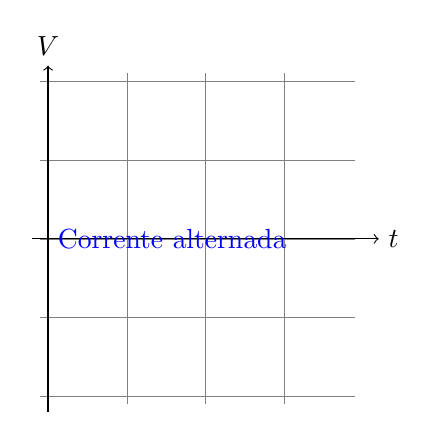
\begin{tikzpicture}[domain=0:4]
        \draw[very thin,color=gray] (-0.1,-2.1) grid (3.9,2.1);
        \draw[->] (-0.2,0) -- (4.2,0) node[right] {$t$};
        \draw[->] (0,-2.2) -- (0,2.2) node[above] {$V$};
        \draw[smooth, color=blue] plot[id=sin] function{sin(5*x)} 
            node[right] {Corrente alternada};
    \end{tikzpicture}1
    }
\caption{\label{fig:corrente-alternada} Característica da corrente alternada}
\end{center}
\end{figure}




% Figura corrente contínua
\begin{figure}[H]
\begin{center}
\fbox {
    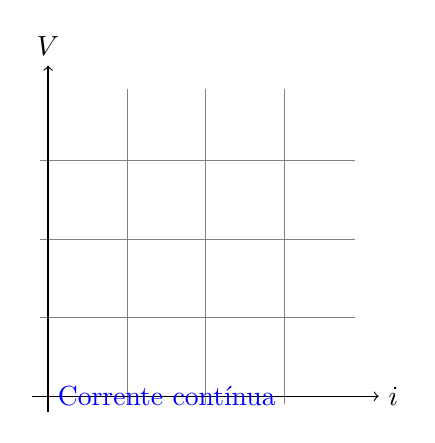
\begin{tikzpicture}[domain=0:4]
        \draw[very thin,color=gray] (-0.1,-0.1) grid (3.9,3.9);
        \draw[->] (-0.2,0) -- (4.2,0) node[right] {$i$};
        \draw[->] (0,-0.2) -- (0,4.2) node[above] {$V$};
        \draw[smooth, color=blue] plot[id=sin] function{2} 
            node[right] {Corrente contínua};
    \end{tikzpicture}
    }
\caption{\label{fig:corrente-continua}Característica da corrente contínua}
\end{center}
\end{figure}

Para época o melhor sistema era o sistema de corrente alternada, porem
se a guerra fosse hoje, provavelmente Thomas Edison teria mais argumentos
que tinha naquela época (onde apenas lampadas eram alimentadas).Hoje
em dia alguns equipamentos utilizam corrente contínua por exemplo:
celular, MP3 player e computador.

Apesar de receber na tomada corrente alternada, precisamos da fonte
que converte corrente alternada em corrente continua, para alimentar
esses aparelhos. Hoje já existem alguns projetos que para diminuir
o custo desses equipamentos ,no qual seria necessário construir uma
fonte, é de utilizar mais corrente continua que corrente alternada.
Se considerarmos que os painéis solares geram em corrente continua,
um cenário onde a guerra entre correntes tende a ficar mais acirrada
no futuro. Se existe uma residencia que possui no telhado geração
de corrente continua e boa parte dos aparelhos consumindo em corrente
continua, as redes de corrente continua passam a ser mais interessantes.

No Brasil existem algumas linhas de corrente continua, atualmente
está sendo construída uma linha que tem origem no norte e chega até
o sudeste.

As linhas de corrente contínua tem custo inicial muito alto, enquanto
as linhas de corrente alternada é crescente . Porem, o custo
de corrente continua diminui com o tempo inclusive considerando as
perdas, no ponto de em torno de 1000Km é mais vantajoso trabalhar
com corrente contínua que com corrente alternada. O custo da corrente
continua é alto justamente pela geração ser em corrente alternada,
então ocorre um trabalho para converter a corrente continua e quanto
chegar no final da linha converter em corrente alternada. Assim, é
possível concluir que com distancias maiores é mais vantajoso trabalhar
com corrente contínua do que com corrente alternada.
\begin{figure}[H]
\begin{centering}
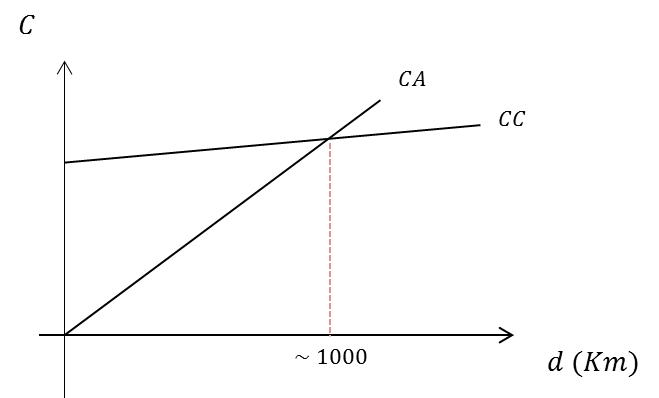
\includegraphics{aula2_3}\protect\caption{\label{fig:aula2_3} Corrente contínua e Corrente alternada }
\end{centering}

\end{figure}

\subsubsection{Sistemas elétricos em corrente alternada}

Os dois equipamentos que permitiram essa revolução e migração da corrente contínua para corrente alternada foram o gerador e o transformador.

Para iniciar o cientista inglês M. Faraday realizou a seguinte experiencia no século XIX, ele pegou uma pilha ,adicionou um chave para ligar e desligar essa pilha e colocou uma bobina com fios enrolados fechando o circuito que não tem nenhuma ligação com a pilha . E do outro lado colocou um aparelho conhecido com galvanômetro ,um aparelho que tem movimento quando ele detecta uma corrente elétrica, o galvanômetro está conecto a uma espira do outro lado. Então, a chave que inicialmente estava aberta foi fechada e  observou uma corrente e dado uma corrente elétrica circulando em uma espira irá aparecer um campo magnético. Faraday percebeu que o fluxo magnético que conecta com o outro lado do experimento gerava uma corrente que o galvanômetro detectava. Um ponto relevante no experimento é que Faraday sabia que corrente provocava fluxo mas não sabia que fluxo provocava corrente. Então esse equipamento movia quando a chave era virada porem depois o equipamento voltava a posição inicial. Quando era desligada a chave, as linhas de fluxos desapareciam e o outro equipamento movia para o outro lado. Assim, quando era ligado o equipamento movimentava-se para um lado e quando desligado o movimento era contrário, invertendo assim o sentido (Figura \ref{fig:aula2_4}). 
\begin{figure}[H]
\begin{centering}
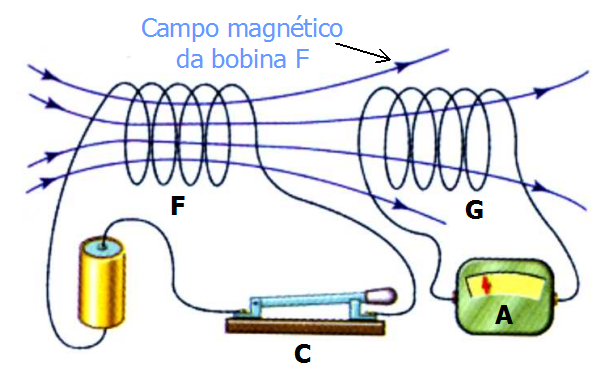
\includegraphics{aula2_4}\protect\caption{\label{fig:aula2_4}Experimento de M.Faraday }
\end{centering}

\end{figure}
Faraday chegou a esse experimento porem quem formulou e explicou porque
o sentido da corrente mudava foi o Lenz que postulou a lei de Lenz.O
experimento de Lenz reproduzir o experimento de M. Faraday só que
ao invés de produzir linhas de fluxos provocados por correntes, foi
colocado um imã. Ele injetou campo magnético na espira, ou seja aproximou
o imã da espira e observou que quando ele aproxima o imã da espira
aparecem linhas de campo de sentido contrário ao movimento que foi
imposto.A medida que ele aproximava apareciam linhas de campos no
sentido contrário e essas linhas de campo induzem a passagem corrente
elétrica nessa espira para recuperar o equilíbrio \ref{fig:aula2_5}. Assim
Lenz (1834) respondeu porque a corrente elétrica mudava de sentido
quando se retirava o campo magnético e segundo a lei de Lenz o sentido
da corrente é oposto da variação do campo magnético que lhe deu origem(Figura \ref{fig:aula2_5}). 
\begin{figure}[H]
\begin{centering}
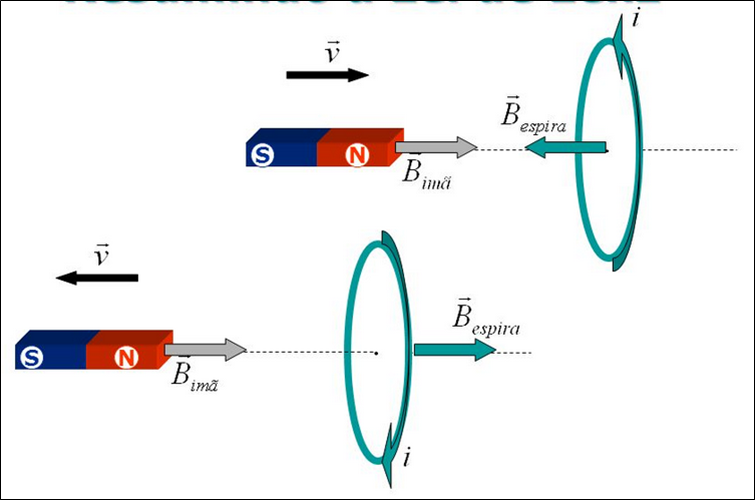
\includegraphics{aula2_5}\protect\caption{\label{fig:aula2_5}Experimento de Lenz }
\end{centering}

\end{figure}

A grandeza escalar que mede o número de linhas de indução que atravessam
a área \textit{\textcolor{black}{A }}de uma espira imersa num campo
magnético uniforme \ref{fig:aula2_6} é chamada fluxo magnético $(\Phi)$, sendo definida
por:
\begin{equation}\label{eq:fluxomag}
\Phi=n\cdot B\cdot A\cdot\cos\theta 
\end{equation}


Dado que,

$A$- área em $m^{2}$

$B$- campo magnético em tesla $(T)$

$\Phi$- fluxo magnético em weber $(Wb)$

$n$- número de espiras.




\begin{figure}[H]
\begin{centering}
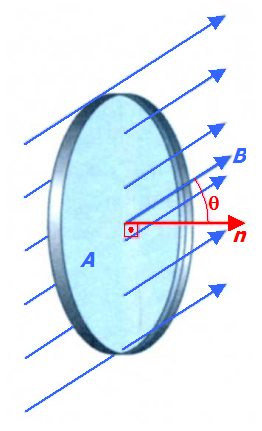
\includegraphics{aula2_6}\protect\caption{\label{fig:aula2_6}Fluxo magnético }
\end{centering}

\end{figure}
Assim, o fluxo magnético será proporcional ao número de espiras,a
intensidade das linhas de campos, a área da seção e o cosseno de $\Theta$
(o angulo entre as linhas de campo magnético e a linha perpendicular
a espira). 

Por exemplo quando $\Theta=0$,fluxo máximo,$\cos\Theta=1$, então
$\Phi=n\cdot B\cdot A$ (Figura \ref{fig:aula2_7}) e quando $\Theta=90^{\circ}$,sem fluxos,$\cos\Theta=0$,
então $\Phi=0$ (Figura \ref{fig:aula2_8}).

\begin{figure}[H]
\begin{centering}
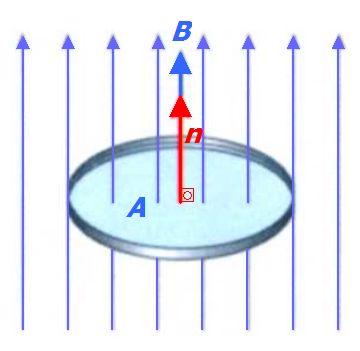
\includegraphics{aula2_7}\protect\caption{\label{fig:aula2_7}Fluxo máximo }
\end{centering}

\end{figure}
\begin{figure}[H]
\begin{centering}
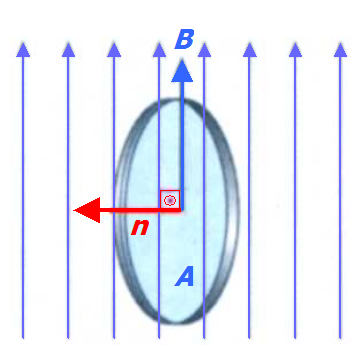
\includegraphics{aula2_8}\protect\caption{\label{fig:aula2_8}Sem fluxo }
\end{centering}

\end{figure}

O outro experimento é ao contrário, deixando o imã fixo e fazer girar
a espira, a experiência é semelhante ,mas trocou a função dos elementos.
Então a geração de energia elétrica será a partir de energia mecânica (Figura
\ref{fig:aula2_9}) . Assim, hora a tensão elétrica é produzida em um sentido, hora
em outro sentido caracterizando a corrente alternada.

\begin{figure}[H]
\begin{centering}
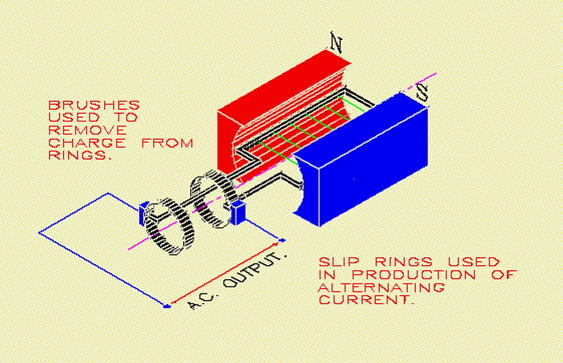
\includegraphics{aula2_9}\protect\caption{\label{fig:aula2_9}Experimento imã fixo }
\end{centering}

\end{figure}

Periodicamente, a variação de fluxo magnético na bobina (girando),
implica em uma tensão variável ao longo do tempo porque em cada hora
a bobina terá uma posição diferente (Figura \ref{fig:aula2_10}). Pela lei de Lenz a hora que injeto
a variação de fluxo no tempo ela produz uma tensão que é contraria
ao movimento que gerou a tensão e a posição da bobina em relação ao
campo magnético depende do tempo. Assim:

\begin{equation}\label{eq:et}
e(t)=\frac{\partial\Phi(t)}{\partial t}
\end{equation}

\begin{figure}[H]
\begin{centering}
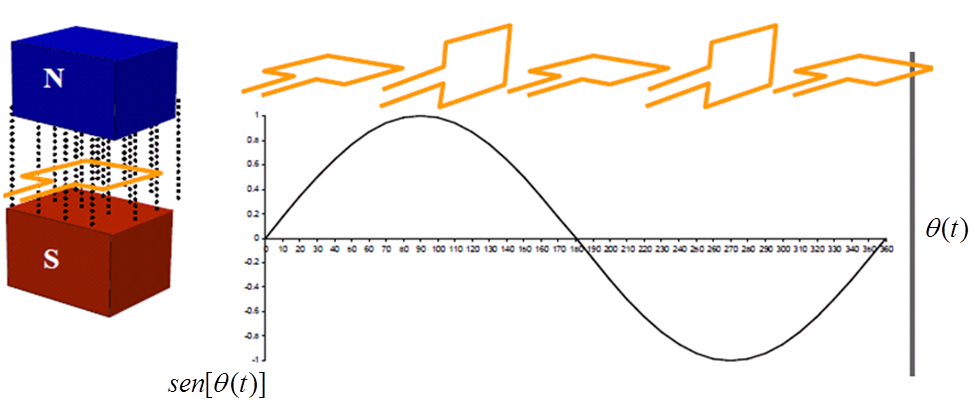
\includegraphics{aula2_10}\protect\caption{\label{fig:aula2_10}A posição da bobina }
\end{centering}

\end{figure}
Definindo $\omega$ como a velocidade angular da bobina. Pode-se escrever:

\begin{equation}\label{eq:omega}
\omega=\frac{\triangle\theta}{\triangle t}(\frac{rad}{seg})
\end{equation}

De outra forma:
\begin{equation}\label{eq:omega2}
\omega=\frac{\theta_{F}-\theta_{I}}{t_{F}-t_{I}}(\frac{rad}{seg})
\end{equation}

Considerando:

$\theta_{I}=0$ e $t_{I}=0$ então:
\begin{equation}\label{eq:omega3}
\omega=\frac{\theta_{F}}{t_{F}}=\frac{\theta}{t}
\end{equation}

Finalmente
\begin{equation}\label{eq:omega4}
\theta=\omega t
\end{equation}
A força eletromotriz $(e)$ em volts pode ser calculada como:

\begin{equation}\label{eq:ele}
e(t)=-\frac{\triangle\Phi(t)}{\triangle t}=-\frac{\partial[nBA\cos(\omega t)]}{\partial t}
\end{equation}

Assim,

$\Phi(t)=nBA\cos(\omega t)$

$e(t)=n\omega BA\sin(\omega t)$

$e(t)=E_{max}\sin(\omega t)$

$E_{max}=n\omega BA$

\begin{figure}[H]
\begin{centering}
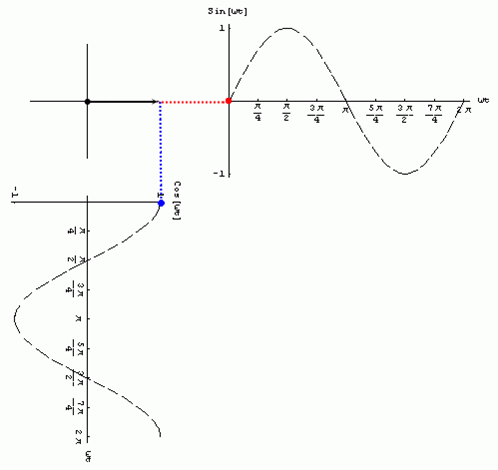
\includegraphics{aula2_11}\protect\caption{\label{fig:aula2_11}A posição da bobina }
\end{centering}

\end{figure}

Na Figura \ref{fig:aula2_11} a tensão e o fluxo variam no tempo.

Definindo $f$ como frequência da rotação. A frequência de rotação
descreve o numero de revoluções (voltas completas) por segundo da
bobina.

Assim,

\begin{equation}\label{eq:freq}
f=\frac{n\text{º revoluções (voltas completas)}}{tempo(seg)}
\end{equation}

A unidade de frequência é hertz. Diz-se que o sistema tem um hertz
se a bobina efetua uma volta completa a cada segundo. No Brasil o
consumo em geral possui um frequência estabelecida de $60$ hertz
ou 377 radianos por segundo. 
A velocidade angular da bobina e, consequentemente, da tensão é ($2\pi$
é uma volta completa):

\begin{equation}\label{eq:omega6}
\omega=\frac{\triangle\theta}{\triangle t}(\frac{rad}{seg})
\end{equation}

De outra forma:
\begin{equation}\label{eq:omega7}
\omega=n\text{º revol.}(\frac{2\pi}{\triangle t})(\frac{rad}{seg})
\end{equation}

Então:
\begin{equation}\label{eq:omega8}
\omega=2\pi f
\end{equation}
Temos que:
\begin{equation}\label{eq:omega9}
\Phi=nBA\cos(2\pi ft)
\end{equation}

\begin{equation}\label{eq:omega10}
\ e(t)=(2\pi f)n\omega BA\sin(2\pi ft)
\end{equation}

\begin{equation}\label{eq:omega11}
[e(t)=E_{max}\sin(2\pi ft)]
\end{equation}
Trabalhar com grandezas no tempo é inconveniente no ponto de vista
matemático, então é comum mudar a forma de trabalhar com as grandezas
no setor elétrico. Já que o sistema elétrico está girando 60 hertz,
então é tirada uma fotografia de um determinado ponto do sistema e
tratar uma grandeza em relação a outra e para isso é necessário estabelecer
uma referencia e ao invés de dizer que estão no domínio do tempo diz-se
que está no domínio da frequência . 

Para evitar a manipulação matemática das grandezas que variam no tempo
criou-se o conceito de fasor, um tipo especial de vetor capaz de representar
uma função sinusoidal. Isto significa que as operações com fasores
são semelhantes às de vetores.

Então a tensão varia com um valor de tensão máxima sendo, $f=A\sin(\omega t+\theta)$.
\begin{figure}[H]
\begin{centering}
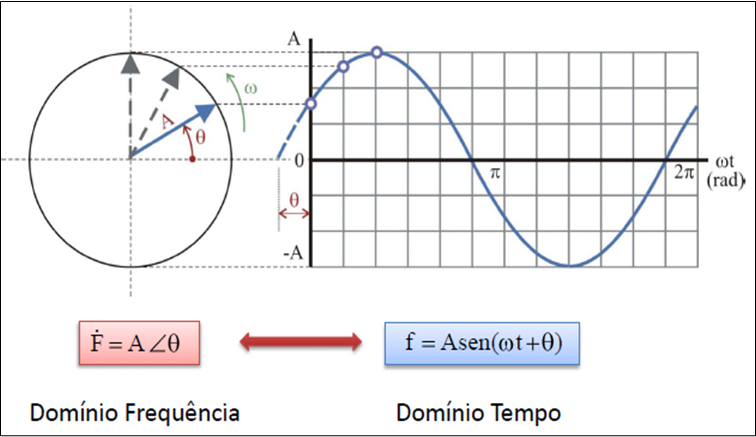
\includegraphics{aula2_12}\protect\caption{\label{fig:aula2_12}Fasores }
\end{centering}
\end{figure}
O que permite de fato levar a energia elétrica de um ponto para outro
ponto muito distante nesse caso ,aumentando a tesão é o transformador
de potencia.

O transformador de potencia é basicamente uma massa de ferro com um
enrolamento (enrola um fio em cada lado) com uma eficiência que é
maior que 90\% ou seja a energia perdida é pequena.

No transformador ideal, a tensão é gerada em função do fluxo magnético
variante no tempo. O fluxo magnético variante no tempo é gerado em
função de uma corrente elétrica variante no tempo.

Se aplicar uma tensão de um lado, a tensão elétrica vai gerar uma
corrente que vai circular, essa corrente vai induzir um fluxo, esse
fluxo que passa no primário concatena com o secundário. Num transformador
ideal todo fluxo concatena. Quando aplica um tensão gera uma corrente
,essa corrente vai produzir um fluxo e no outro lado se conectar uma
carga vai aparecer uma corrente elétrica.
\begin{figure}[H]
\begin{centering}
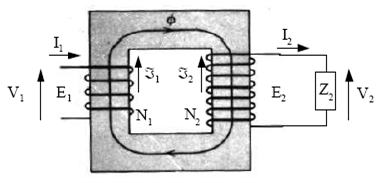
\includegraphics{aula2_13}\protect\caption{\label{fig:aula2_13}Transformador ideal de potência}
\end{centering}
\end{figure}

Matematicamente, da Lei de Faraday:
\begin{equation}\label{eq:lf}
\dot{\dot{V}_{1}=-N_{1}\frac{d\Phi}{dt}}
\end{equation}
\begin{equation}\label{eq:lf2}
\dot{\dot{V}_{2}=-N_{2}\frac{d\Phi}{dt}}
\end{equation}


Sendo:
$\dot{V_{i}}:$ Tensão (fasorial) no terminal i;

$\dot{I_{i}}:$ Tensão (fasorial) no terminal i;

$\dot{Ni}:$ Número de espiras no terminal i;

$\frac{d\Phi}{dt}$: Fluxo magnético variante no tempo.

Assim,

\begin{equation}\label{eq:lf2}
\frac{\dot{V}_{1}}{\dot{V}_{2}}=\frac{N_{1}}{N_{2}}=\alpha
\end{equation}

$\alpha$: Relação de transformação.

Se por exemplo colocarmos 10 espiras no primário e uma espira no secundário,eleva
a tensão no secundário para 10 vezes do primário. 

O análogo magnéticos (Figura \ref{fig:aula2_14}) do circuito elétrico do transformador:
\begin{equation}\label{eq:cet1}
\Im_{1}-\Im_{2}=\Re\cdot\Phi
\end{equation}

\begin{equation}\label{eq:cet2}
\Im_{1}=N_{1}\cdot\dot{I}_{1}
\end{equation}

\begin{equation}\label{eq:cet3}
\Im_{2}=N_{2}\cdot\dot{I}_{2}
\end{equation}


Onde, 

$\Im_{i}$- Força magnetomotriz no terminal $i$ (A.e);

$\Phi$- Fluxo magnético induzido (Wb);

$\Re$- Relutância do transformador (A/Wb).

No transformador ideal, a relutância é nula. Assim:

\begin{equation}\label{eq:cet4}
N_{1}\cdot\dot{I}_{1}=N_{2}\cdot\dot{I}_{2}\rightarrow\frac{\dot{I}_{1}}{\dot{I}_{2}}=\frac{N_{1}}{N_{2}}=\frac{1}{\alpha}\rightarrow\dot{I}_{1}=\frac{1}{\alpha}\cdot\dot{I}_{2}
\end{equation}

\begin{figure}[H]
\begin{centering}
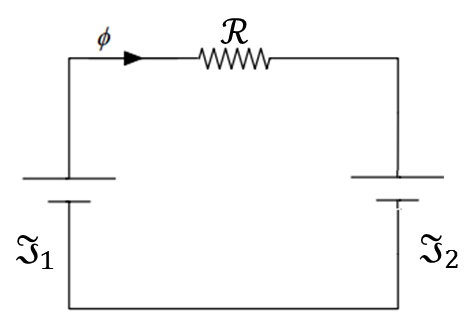
\includegraphics{aula2_14}\protect\caption{\label{fig:aula2_14}Circuito Magnético}
\end{centering}
\end{figure}

Ps: O transformador permite reduzir a corrente elétrica nas linhas
de transmissão aumentando a tensão. Neste caso, a energia elétrica
pode ser transmitida a grandes distâncias com menores perdas. 







\subsection{Evolução dos Sistemas Elétricos}


No nosso dia a dia, no trabalho, nos estudos, no lazer, sempre estamos fazendo uso da energia elétrica. A maioria das pessoas, no entanto, dão pouca importância para como esta energia chega até elas. Bom, o leite não vem da caixinha do supermercado, da mesma forma que a energia não chega magicamente às tomadas das nossas casas. Um sistema elétrico é algo muito complexo e que requer muito cuidado e planejamento. Imagine todo o Brasil interligado por uma rede de linhas de transmissão, com inúmeras unidades de geração e milhões de pessoas consumindo energia ao mesmo tempo. Quem controla tudo isso? Quem garante que a energia chegue às nossas casas? Se uma linha para de funcionar, como fazemos para levar a energia ao seu destino sem sobrecarregar demais as outras linhas?


Um sistema elétrico pode ser dividido em três partes: 1) Geração; 2) Transmissão; 3) Distribuição. A figura \ref{fig:sist} mostra um exemplo de um sistema elétrico. Tudo começa nas geradoras, que podem ser hidroelétricas, termoelétricas, torres eólicas, usinas nucleares e outras. A energia gerada vai para uma rede de transmissão básica que leva a energia até as estações de distribuição, para só então a energia chega ao consumidor final, nos famosos 110 (ou, à rigor, 127) e 220 volts que conhecemos. 

\begin{figure}[h]
\begin{centering}
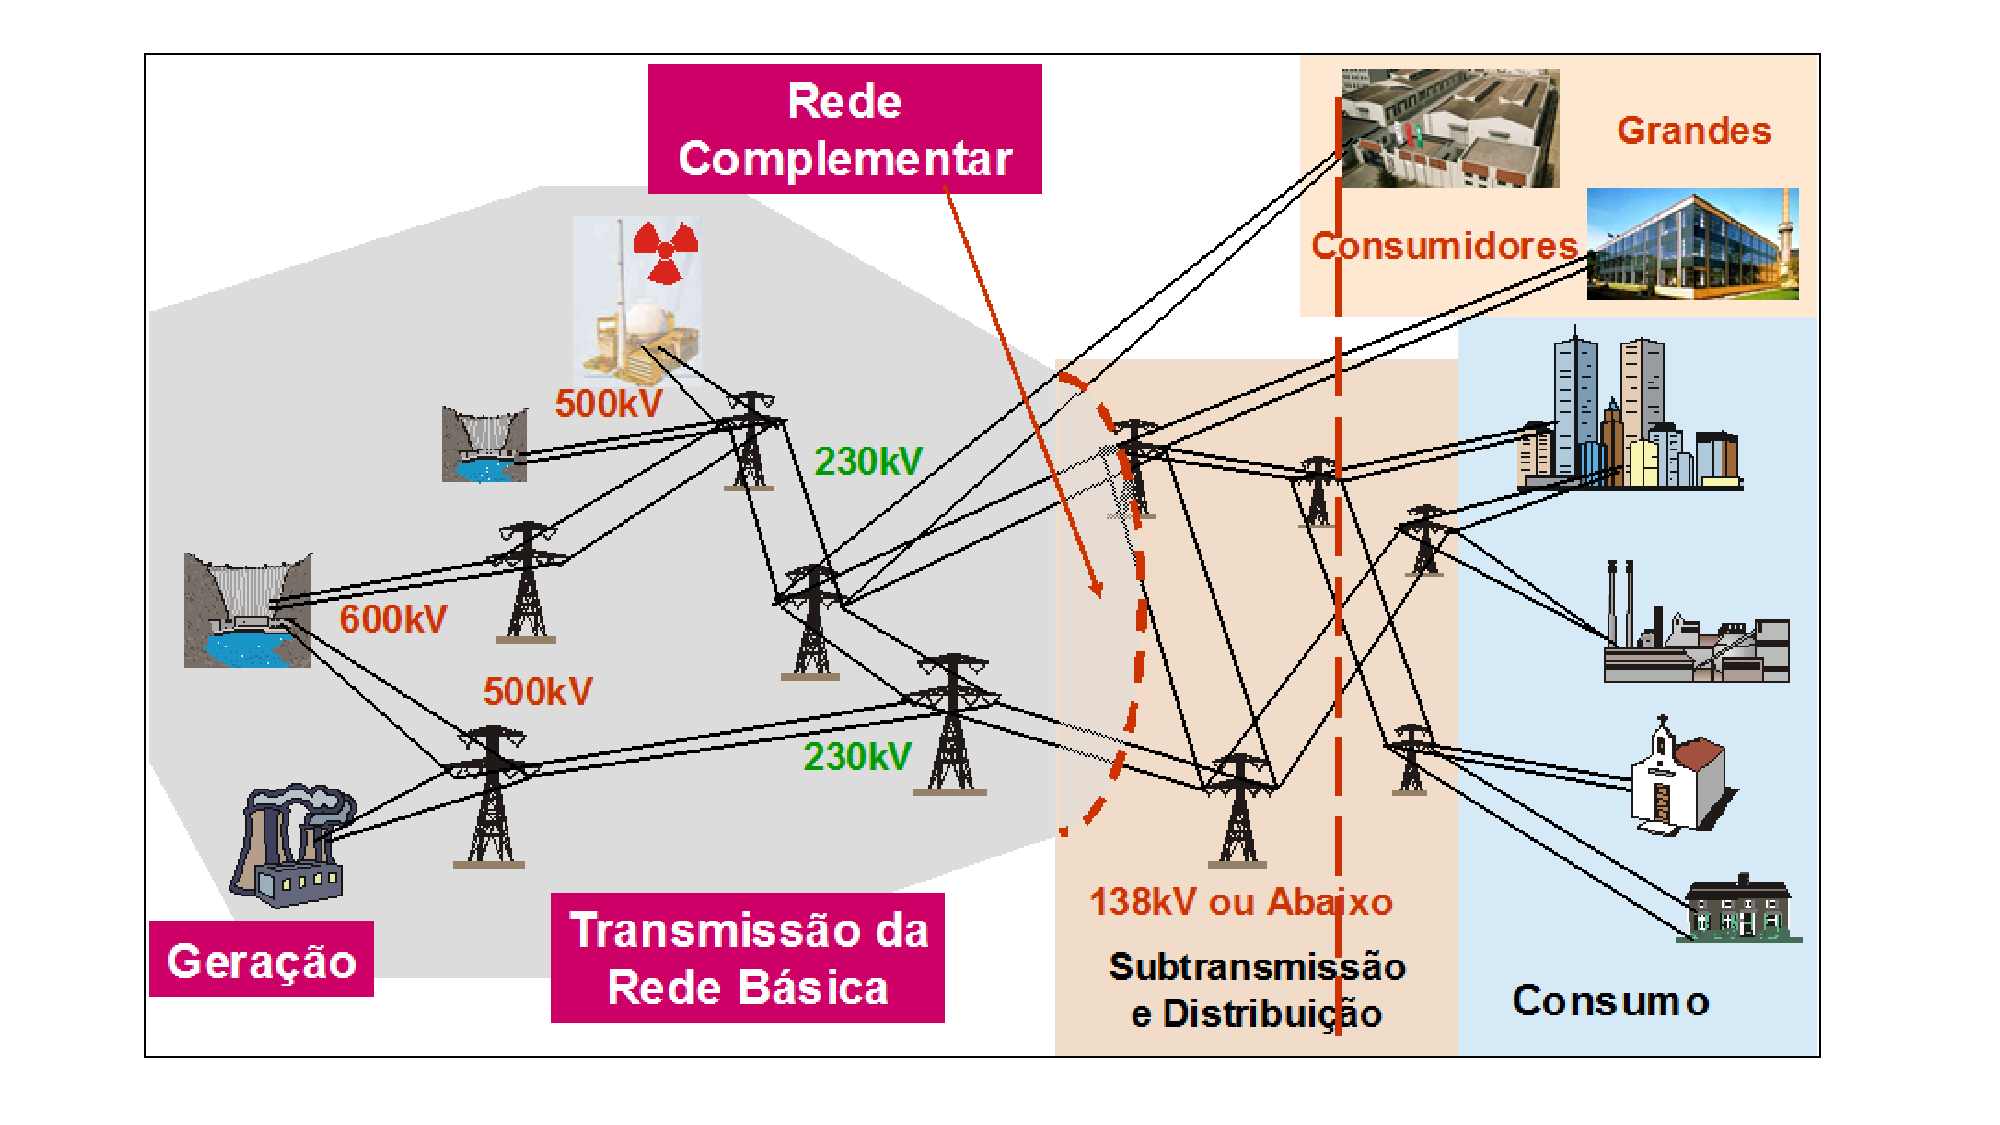
\includegraphics[scale=0.5]{anexos/figsist}
\par\end{centering}

\caption{\label{fig:sist}Representação de um sistema elétrico}
\end{figure}

\begin{figure}[h]
\begin{centering}
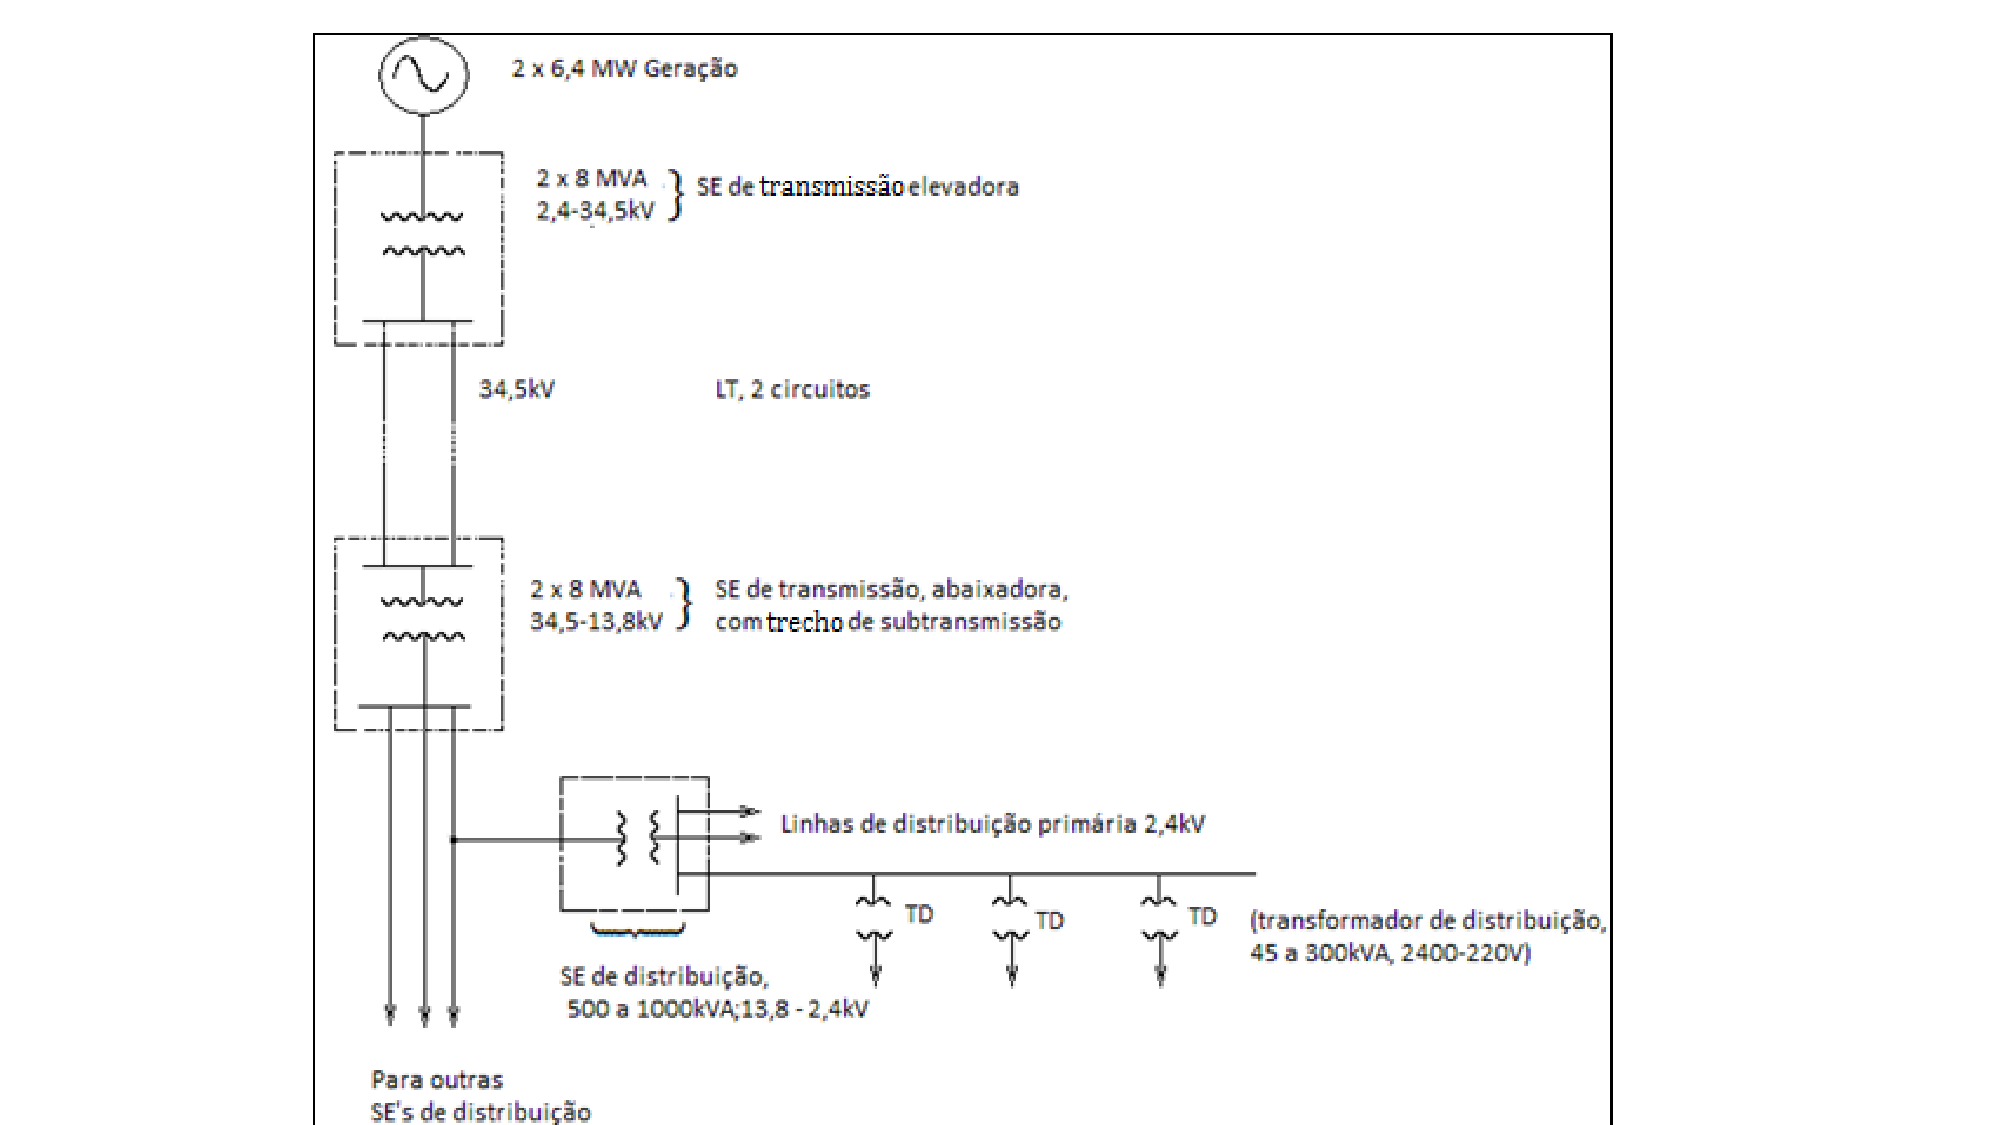
\includegraphics[scale=0.5]{anexos/figrede}
\par\end{centering}

\caption{\label{fig:rede}Sistema elétrico pequeno isolado}
\end{figure}

A figura \ref{fig:rede} mostra um pequeno sistema elétrico. As linhas e subestações no sistema são classificadas pela transformação no nível de tensão, e não a tensão no sistema como um todo. Pela figura podemos ver a tensão da geradora, que é aumentada em uma subestação. Em seguida, temos outra subestação que abaixa a tensão para 13.8kV até chegar subestação que leva às linhas de distribuição primárias, a 2.4kV. Estas linhas levam a energia até o poste, que tem um transformador que faz a energia chegar em nossas casas na tensão desejada, por exemplo, 220V. 

Já deu para notar que um sistema elétrico não é uma coisa simples, e que exige muita sincronia. Para controlar tudo isso existe o \textbf{Operador do Sistema}, que é uma entidade, que pode ou não pertencer ao governo, responsável por assegurar a funcionalidade do sistema elétrico. Dentre a funções do Operador do Sistema estão: garantir o funcionamento do mercado de energia (se ele existir), manter o sistema na frequência utilizada, assegurar que a demanda de energia será suprida, auxiliar no planejamento de expansão do sistema, minimizar custos de operação, entre outras. Estas funções podem variar de país para país.

Vamos falar agora sobre os diferentes custos de um sistema elétrico e como eles são classificados. Em primeiro lugar temos o custo de geração, que pode variar muito de gerador para gerador tanto em estrutura quando em valores absolutos. A construção de uma hidroelétrica é muito cara; entretanto, uma vez construída, a água não custa nada, ou seja, a usina não paga quase nada para funcionar. Em uma escala menor, o mesmo é valido para um parque eólico. No outro extremo estão as usinas térmicas; elas geralmente são baratas para serem construídas e podem ficar em qualquer lugar, o que reduz o custo de transmissão. No entanto, elas precisam queimar algum combustível como carvão ou gás natural, ou seja, apesar de serem baratas para construir, elas custam muito para operar. O primeiro caso que apresentamos foi o de geradores com um alto \textbf{custo fixo} e um baixo \textbf{custo variável}, no segundo caso esta relação se inverte. Além dos custos citados acima, fazem parte dos custos de geração possível custos ancilares, que podem ser custos da reserva de potência ativa, reativa, controle de frequência, controle de congestionamento do sistema, auto-restabelecimento, controle de tensão e outros.

Saindo da geração, vamos para os custos de transmissão e distribuição. Em primeiro lugar, quem arca com estes custos? Todos nós usamos linhas de transmissão, portanto o rateio destes custos pode ser algo complicado. Os custos de transmissão e distribuição são basicamente de construção e manutenção, no entanto, perdas de energia no sistema também são consideradas. É natural esperar que alguma energia será perdida no processo, e cabe ao planejador do sistema elétrico tentar minimizar estas perdas. 



\subsection{Modelagem dos Sistemas Elétricos}

Nesta seção, apresentaremos os três elementos utilizados para modelar as linhas de transmissão: resistores, indutores e capacitores. Veremos como a aplicação de uma tensão alternada se relaciona com a corrente gerada em cada um dos elementos. 

\subsubsection*{Resistores}


\begin{figure}
    \centering
    \begin{subfigure}[b]{0.3\textwidth}
        \centering
        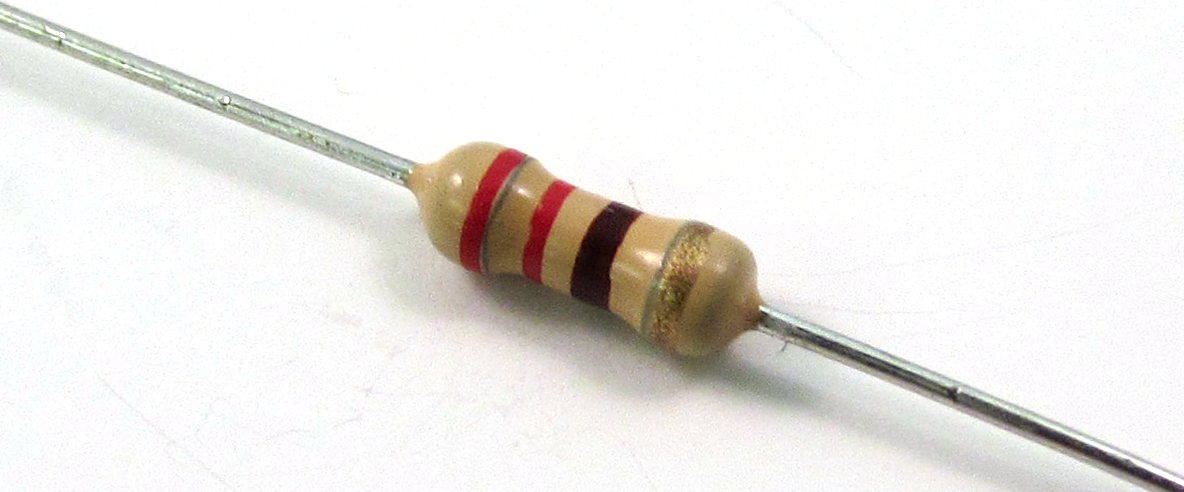
\includegraphics[width=\textwidth]{anexos/resistor.png}
        %\caption{$y=x$}
        %\label{fig:y equals x}
    \end{subfigure}
    \hspace{1cm}
    \begin{subfigure}[b]{0.3\textwidth}
        \centering
        \fbox{
            \begin{circuitikz} \draw
            (0,0) to[R, o-o, l=R] (0,2.5)
            ;
            \end{circuitikz}%\caption{$y=3sinx$}
            }
        %\label{fig:three sin x}
    \end{subfigure}
    

    \caption{À esquerda, um resistor real. À direita, a representação esquemática de um resistor.}
    \label{fig:three graphs}
\end{figure}


São equipamentos com características resistivas, como chuveiro elétrico
e aquecedor. As equações para a tensão ($V$) e corrente ($i$) em
função do tempo, assim como a representação com seus fasores correspondentes,
são exibidas a seguir:

\[
i(t)=\frac{V_{m}}{R}\mbox{\, sen}(wt+\phi)\qquad\longrightarrow\qquad\dot{I}=\frac{V_{m}}{R}\angle\phi^{\circ},
\]


\[
V(t)=V_{m}\mbox{\, sen}(wt+\phi)\qquad\longrightarrow\qquad\dot{V}=V_{m}\angle\phi^{\circ},
\]
em que $V_{m}$ é o valor máximo da tensão, ou seja, a sua amplitude.
A notação de fasor é uma forma simplificada de determinar a grandeza
no tempo, sem ter que especificar a função no sentido temporal, desde
que a frequência seja a mesma para todas as funções. No sistema elétrico utiliza-se comumente
frequências entre 50 e 60Hz. No Brasil, o padrão é de 60Hz. 

Para um resistor tem-se no domínio do tempo que 
\[
V(t)/i(t)=\frac{\frac{V_{m}}{R}\mbox{\, sen}(wt+\phi)}{V_{m}\mbox{\, sen}(wt+\phi)}=R
\]
 e no domínio da frequência que 
\[
\dot{V}/\dot{I}=R.
\]
 Assim, a fase que a corrente se encontra é exatamente a mesma da
tensão, como mostra a figura \ref{fig:fase-ct-resistor}. Como será
visto a seguir, isto não acontece para indutores e capacitores.



%\begin{center}
%\begin{table}[H]
%\begin{tabular}{ll}
%\multirow{2}{5cm}{  \begin{circuitikz} \draw
%    (0,0) to[R, o-o, l=R] (0,3)
%    ;
%    \end{circuitikz}}    & $e = E_m\text{sen}(wt+\phi)$ \\
%                                        & $i=\dfrac{E_m}{R}\text{sen}(wt+\phi)$ \\
%\end{tabular}
%\end{table}
%\end{center}

%\begin{figure}[H]
%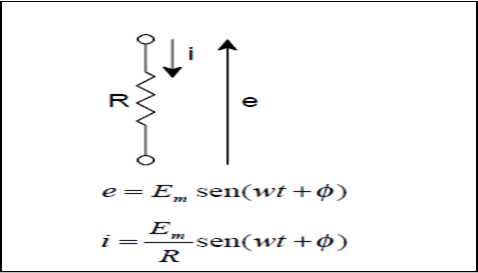
\includegraphics{anexos/aula2_1.png}\protect\caption{Resistores}
%\end{figure}




%Figura resistor
\begin{figure}[H]
\begin{center}
\fbox {
    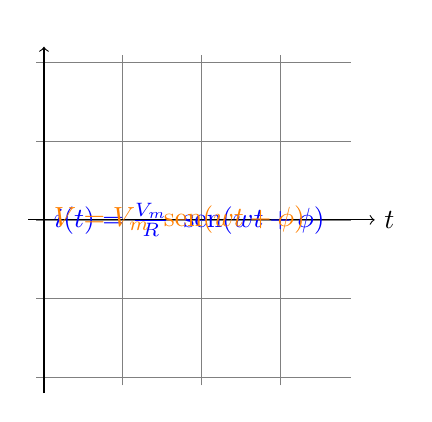
\begin{tikzpicture}[domain=0:4]
        \draw[very thin,color=gray] (-0.1,-2.1) grid (3.9,2.1);
        \draw[->] (-0.2,0) -- (4.2,0) node[right] {$t$};
        \draw[->] (0,-2.2) -- (0,2.2) node[above] {};
        \draw[smooth, color=blue] plot[id=sin] function{sin(5*x)} 
            node[right] {$i(t)=\frac{V_{m}}{R}\mbox{\,\ sen}(wt+\phi)$};
        \draw[smooth, color=orange] plot[id=exp] function{2*sin(5*x)} 
            node[right] {$V=V_{m}\mbox{\, sen}(wt+\phi)$};
    \end{tikzpicture}
    }
\caption{\label{fig:fase-ct-resistor}Corrente e tensão oscilam na mesma fase no resistor}
\end{center}
\end{figure}


\subsubsection*{Indutores}

% Figura Indutor
\begin{figure}
    \centering
    \begin{subfigure}[b]{0.3\textwidth}
        \centering
        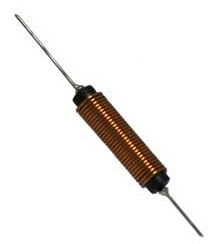
\includegraphics[width=\textwidth]{anexos/indutor.png}
        %\caption{$y=x$}
        %\label{fig:y equals x}
    \end{subfigure}
    \hspace{1cm}
    \begin{subfigure}[b]{0.3\textwidth}
        \centering
        \fbox{
            \begin{circuitikz} \draw
            (0,0) to[cute inductor, o-o, l=L] (0,2.5)
            ;
            \end{circuitikz}%\caption{$y=3sinx$}
            }
        %\label{fig:three sin x}
    \end{subfigure}
    \caption{À esquerda, um indutor real. À direita, a representação esquemática de um indutor.}
    \label{fig:three graphs}
\end{figure}


Quando a corrente passa por equipamentos como um motor elétrico ou
um transformador (elementos indutivos), a fase da corrente se atrasa
com relação à tensão. Sendo a diferença de potencial num indutor medido
como $V=L\,\frac{di}{dt}$, em que $L$ é a indutância, apresentamos a seguir o cálculo das relações
entre corrente e tensão a seguir:

\[
i(t)=\frac{V_{m}}{R}\mbox{\,\ sen}(wt+\phi)\qquad\longrightarrow\qquad\dot{I}=I_{m}\angle\phi^{\circ},
\]


\[
V(t)=L\,\frac{di}{dt}=wLI_{m}\mbox{cos}(wt+\phi)=wLI_{m}\mbox{sen}(wt+\phi+90)\qquad\longrightarrow\qquad\dot{V}=wLI_{m}\angle\phi+90^{\circ},
\]


\begin{equation}
\frac{\dot{V}}{\dot{I}}=\frac{wLI_{m}\angle\phi+90^{\circ}}{I_{m}\angle\phi^{\circ}}=wL\angle90^{\circ}.\label{eq:fase-v-i}
\end{equation}
Assim, conforme visto nas equações acima, a fase da corrente num indutor
se atrasa em $90^{\circ}$ com relação à tensão. A forma regular da
expressão \ref{eq:fase-v-i} pode ser escrita também como um número
complexo num plano de Argand-Gauss: 
\[
\frac{\dot{V}}{\dot{I}}=jwL.
\]
Este plano é similar ao plano cartesiano, com a diferença que no eixo horizontal está a parte real $a$ do número $a+bj$ e no eixo vertical a parte imaginária $b.$ Nota-se que utiliza-se a letra $j$ para representar $\sqrt{-1}$, pois a letra $i$ já é usada para denominar a corrente. Denomina-se como \textbf{reatância indutiva} ($X_L$)o valor equivalente de resistência que o indutor provoca no sistema. 



% Figura senoide Indutor
\begin{figure}[H]
\begin{center}
\fbox {
    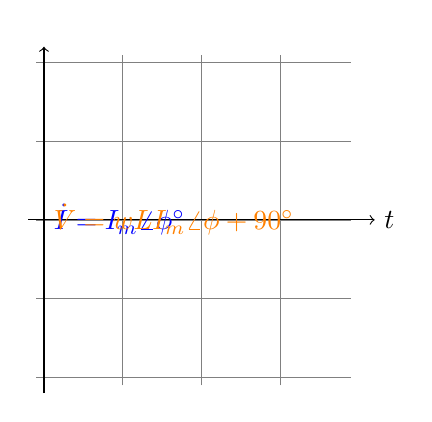
\begin{tikzpicture}[domain=0:4]
        \draw[very thin,color=gray] (-0.1,-2.1) grid (3.9,2.1);
        \draw[->] (-0.2,0) -- (4.2,0) node[right] {$t$};
        \draw[->] (0,-2.2) -- (0,2.2) node[above] {};
        \draw[smooth, color=blue] plot[id=sin] function{sin(6*x)} 
            node[right] {$\dot{I}=I_{m}\angle\phi^{\circ}$};
        \draw[smooth, color=orange] plot[id=exp] function{2*sin(6*x+90)} 
            node[right] {$\dot{V}=wLI_{m}\angle\phi+90^{\circ}$};
    \end{tikzpicture}
    }
\caption{\label{fig:fase-ct-indutor}Corrente é atrasada em 90º com relação à tensão num indutor}
\end{center}
\end{figure}


\subsubsection*{Capacitores}

%Figura capacitor 
\begin{figure}
    \centering
    \begin{subfigure}[b]{0.3\textwidth}
        \centering
        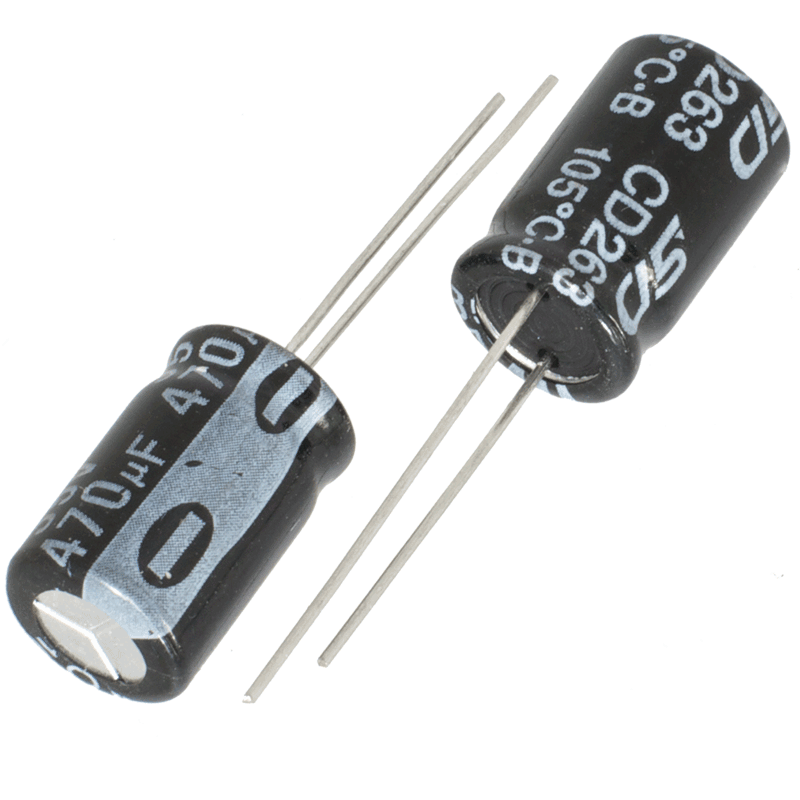
\includegraphics[width=\textwidth]{anexos/capacitor.png}
        %\caption{$y=x$}
        %\label{fig:y equals x}
    \end{subfigure}
    \hspace{1cm}
    \begin{subfigure}[b]{0.3\textwidth}
        \centering
        \fbox{
            \begin{circuitikz} \draw
            (0,0) to[capacitor, o-o, l=C] (0,2.5)
            ;
            \end{circuitikz}%\caption{$y=3sinx$}
            }
        %\label{fig:three sin x}
    \end{subfigure}
    \caption{À esquerda, um resistor real. À direita, a representação esquemática de um resistor.}
    \label{fig:three graphs}
\end{figure}


O único elemento capacitivo numa rede são os próprios bancos de capacitores.
Ele é utilizado principalmente para regulagem da tensão e fator de
potência. Sendo $C$ a capacitância do capacitor em questão, temos
que:

\[
V(t)=V_{m}\mbox{\,\ sen}(wt+\phi)\qquad\longrightarrow\qquad\dot{V}=V_{m}\angle\phi^{\circ},
\]


\[
i(t)=C\,\frac{dV}{dt}=wCV_{m}\mbox{cos}(wt+\phi)=wCV_{m}\,\mbox{sen}(wt+\phi+90)\qquad\longrightarrow\qquad\dot{I}=wCV_{m}\angle\phi+90^{\circ},
\]


\[
\frac{\dot{V}}{\dot{I}}=\frac{V_{m}\angle\phi^{\circ}}{wCV_{m}\angle\phi+90^{\circ}}=\frac{1}{wC\angle90^{\circ}}.
\]
Passando para a forma retangular através de números complexos, temos que
\[
\frac{\dot{V}}{\dot{I}}=\frac{1}{jwC}=\frac{-j}{wC}.
\]
Assim, a reatância capacitiva é dada por $X_{C}=\frac{1}{wC}$. 

% Figura capacitor
\begin{figure}[H]
\begin{center}
\fbox {
    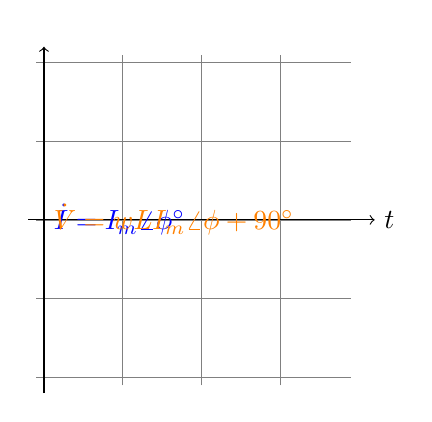
\begin{tikzpicture}[domain=0:4]
        \draw[very thin,color=gray] (-0.1,-2.1) grid (3.9,2.1);
        \draw[->] (-0.2,0) -- (4.2,0) node[right] {$t$};
        \draw[->] (0,-2.2) -- (0,2.2) node[above] {};
        \draw[smooth, color=blue] plot[id=sin] function{sin(5*x)} 
            node[right] {$\dot{I}=I_{m}\angle\phi^{\circ}$};
        \draw[smooth, color=orange] plot[id=exp] function{2*sin(5*x-90)} 
            node[right] {$\dot{V}=wLI_{m}\angle\phi+90^{\circ}$};
    \end{tikzpicture}
    }
\caption{\label{fig:fase-ct-indutor}Corrente é adiantada em 90º com relação à tensão num capacitor}
\end{center}
\end{figure}

\subsubsection*{Linhas de transmissão}

Para modelar as linhas de transmissão, verifica-se qual a impedância do sistema. A impedância é dada pela combinação da resistência, reatância capacitiva e reatância indutiva.

% Figura corrente alternada
%\begin{figure}[H]
%\begin{center}
%\fbox {
%    \begin{tikzpicture}[domain=0:4]
%        \draw[very thin,color=gray] (-0.1,-2.1) grid (3.9,2.1);
%        \draw[->] (-0.2,0) -- (4.2,0) node[right] {$t$};
%        \draw[->] (0,-2.2) -- (0,2.2) node[above] {$V$};
%        \draw[smooth, color=blue] plot[id=sin] function{sin(5*x)} 
%            node[right] {Corrente alternada};
%    \end{tikzpicture}
%    }
%\caption{\label{fig:fase-ct-indutor}Corrente é atrasada em 90º com relação à tensão num indutor}
%\end{center}
%\end{figure}
%
%
%
%
%% Figura corrente contínua
%\begin{figure}[H]
%\begin{center}
%\fbox {
%    \begin{tikzpicture}[domain=0:4]
%        \draw[very thin,color=gray] (-0.1,-0.1) grid (3.9,3.9);
%        \draw[->] (-0.2,0) -- (4.2,0) node[right] {$i$};
%        \draw[->] (0,-0.2) -- (0,4.2) node[above] {$V$};
%        \draw[smooth, color=blue] plot[id=sin] function{2} 
%            node[right] {Corrente contínua};
%    \end{tikzpicture}
%    }
%\caption{\label{fig:fase-ct-indutor}Corrente é atrasada em 90º com relação à tensão num indutor}
%\end{center}
%\end{figure}
%
%
%
%\begin{center}
%\begin{tikzpicture}
%    \begin{axis}[domain=0:1,legend pos=outer north east]
%    \addplot[smooth] {2*sin(20*deg(x))}; 
%    \addplot[smooth, red] {sin(20*deg(x))}; 
%    \legend{$i=\frac{E_{m}}{R}\mbox{\,\ sen}(wt+\phi)$,$
%e=E_{m}\mbox{\, sen}(wt+\phi)$}
%    \end{axis}
%\end{tikzpicture}
%\end{center}
